\chapter[Object and Event Selection][Object and Event Selection]{Object and Event Selection}
\label{chapter:selection}

The analysis is divided into 3 signal regions based
on lepton counting: 2 same-sign leptons, 3 leptons and 4 leptons. The lepton
counting occurs for fully identified leptons with full overlap removal with
transverse momenta over 10 \gev\ to ensure orthogonality. Lepton selections are tightened
afterward within each region.

The cuts for each signal region are provided in Table \ref{table:selection} and the object selections are detailed in the
following selections. The selections are based on optimizations of the region sensitivity
performed using MC (event for data driven backgrounds) and ad-hoc values for normalization systematic uncertainties\footnote{the sensitivity was approximated using the $\frac{s}{\sqrt{b + \Delta b}}$ formula. The systematic errors considered were 20\% for \ttV\ and $VV$ and 30\% for fakes. These ended up being close the final systematic errors assessed in Chapter~\ref{chapter:systematics}. The objects of optimization were the lepton momenta, identification operating points, isolation and event kinematic variables} 

All signal regions are comprised of three basic requirements: the presence of b-tagged
jets, the presence of additional light jets, and a veto of same flavor opposite sign leptons with an
invariant mass within the Z window. Additional requirements on the invariant mass of the leptons, the missing transverse energy
in the event, and the total object energy ($\rm H_{T}$) proved to have negligible additional benefit at our level of 
statistics. Figure~\ref{figure:selection} shows the background and signal fractions as a function number of jets and 
number of b-tagged jets for otherwise fully selected events. 

\begin{table}[htbp]
  \begin{center} 
    \caption{Selections in the 2$\ell$ SS, 3$\ell$ and 4$\ell$ Signal Regions}
      \label{table:selection}
   {\small
    \begin{tabular}{|l|c|c|c|} 
  
  \hline 
  Signal Region   & 2$\ell$ SS & 3$\ell$  & 4$\ell$ \\\hline\hline
  Trigger Matched Lepton   & Yes & Yes    & Yes \\ \hline
  N$_{l}$\footnote{lepton counting is for \pt $=$ 10 GeV leptons, based on the standard criteria outlined in the sections that follow}& $=$2, $N_{\tau}=0$&  $=$3       & $=$4 \\\hline
  Lepton Charge Sum & $+$2 or $-$2     & $+$1 or $-$1 & 0 \\ \hline
  Lepton Momentum (GeV)\footnote{lepton (0,1,2,3) are \pt ordered, with the exception of the 3$\ell$ case} & \pt$_0>$ 25   &  \pt$_0>$ 10 & \pt$_0>$ 25   \\
  & \pt$_1 >$ 20 &  \pt$_{1,2}>$25,20 & \pt$_1>$ 20 \\
  &                   &                          &  \pt$_{2,3}>$ 10 \\\hline
  Jet Counting    & N$_{b}\geq 1$, N$_{Jet} =$  4 & N$_{b}\geq 1$, N$_{Jet} \geq$ 4 & N$_{b}\geq 1$, N$_{Jet} \geq$ 2   \\
                  &                               &        or N$_{b}\geq 2$, N$_{Jet} =$ 3         &                                   \\\hline
  Mass Variables (GeV) &   &  $|M_{SFOS}-M_Z| <$ 10  &  $M_{SFOS} >$ 10   \\
  &   &     & $150 <M_{4\ell} <500$    \\
  &   &     & $|M_{SFOS}-M_Z| <$ 10     \\\hline
  Sub-channels     & 2 (N$_{Jet}=4$, N$_{Jet}\geq$ 5) &  none  &  2 (No SFOS leps,    \\
  &  x 3(ee,e$\mu$,$\mu\mu$)  &     & SFOS leps)    \\\hline
    \end{tabular}} 
  \end{center}
\end{table}

\begin{figure}[!t]
\centering
\begin{tabular}{ccc}
\subfloat[2$\ell$ SS]{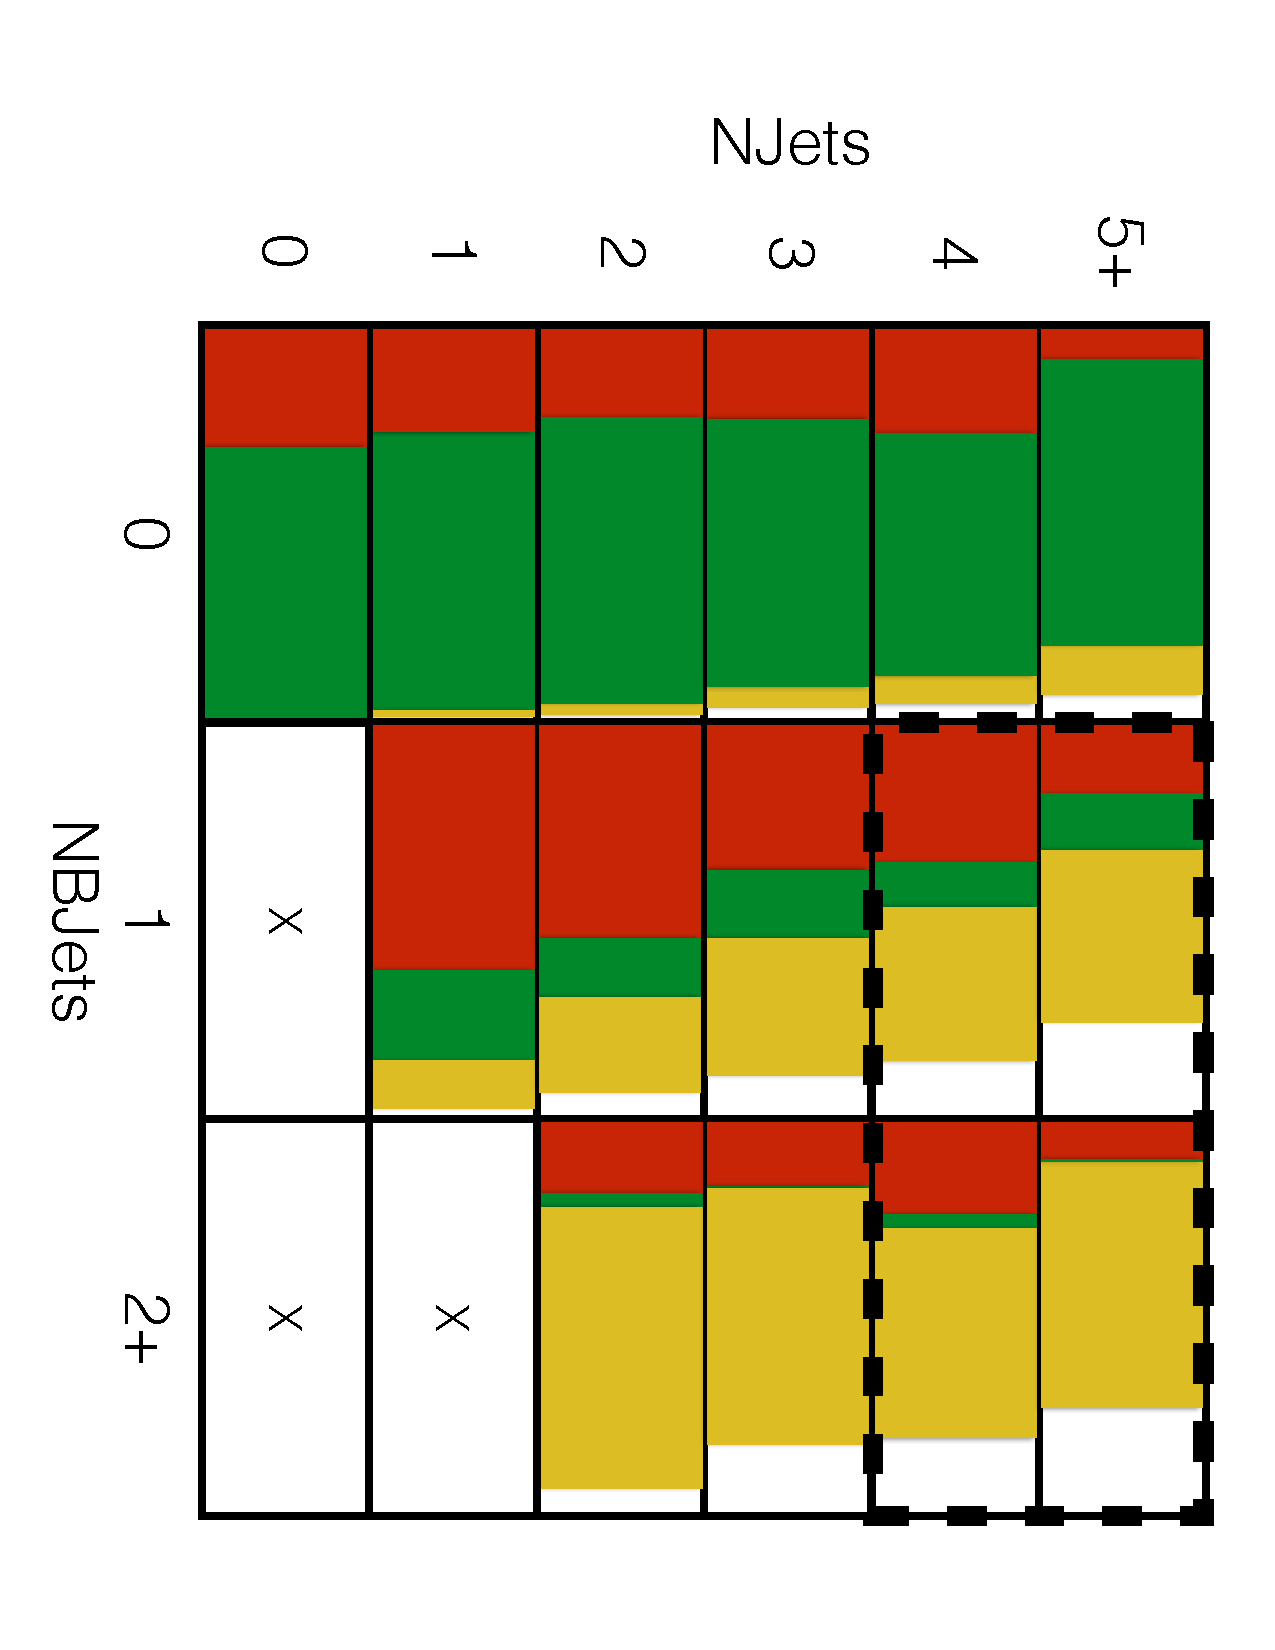
\includegraphics[angle=90,width=0.32\textwidth]{figs/selection/2l_selection.pdf}} &
\subfloat[3$\ell$]{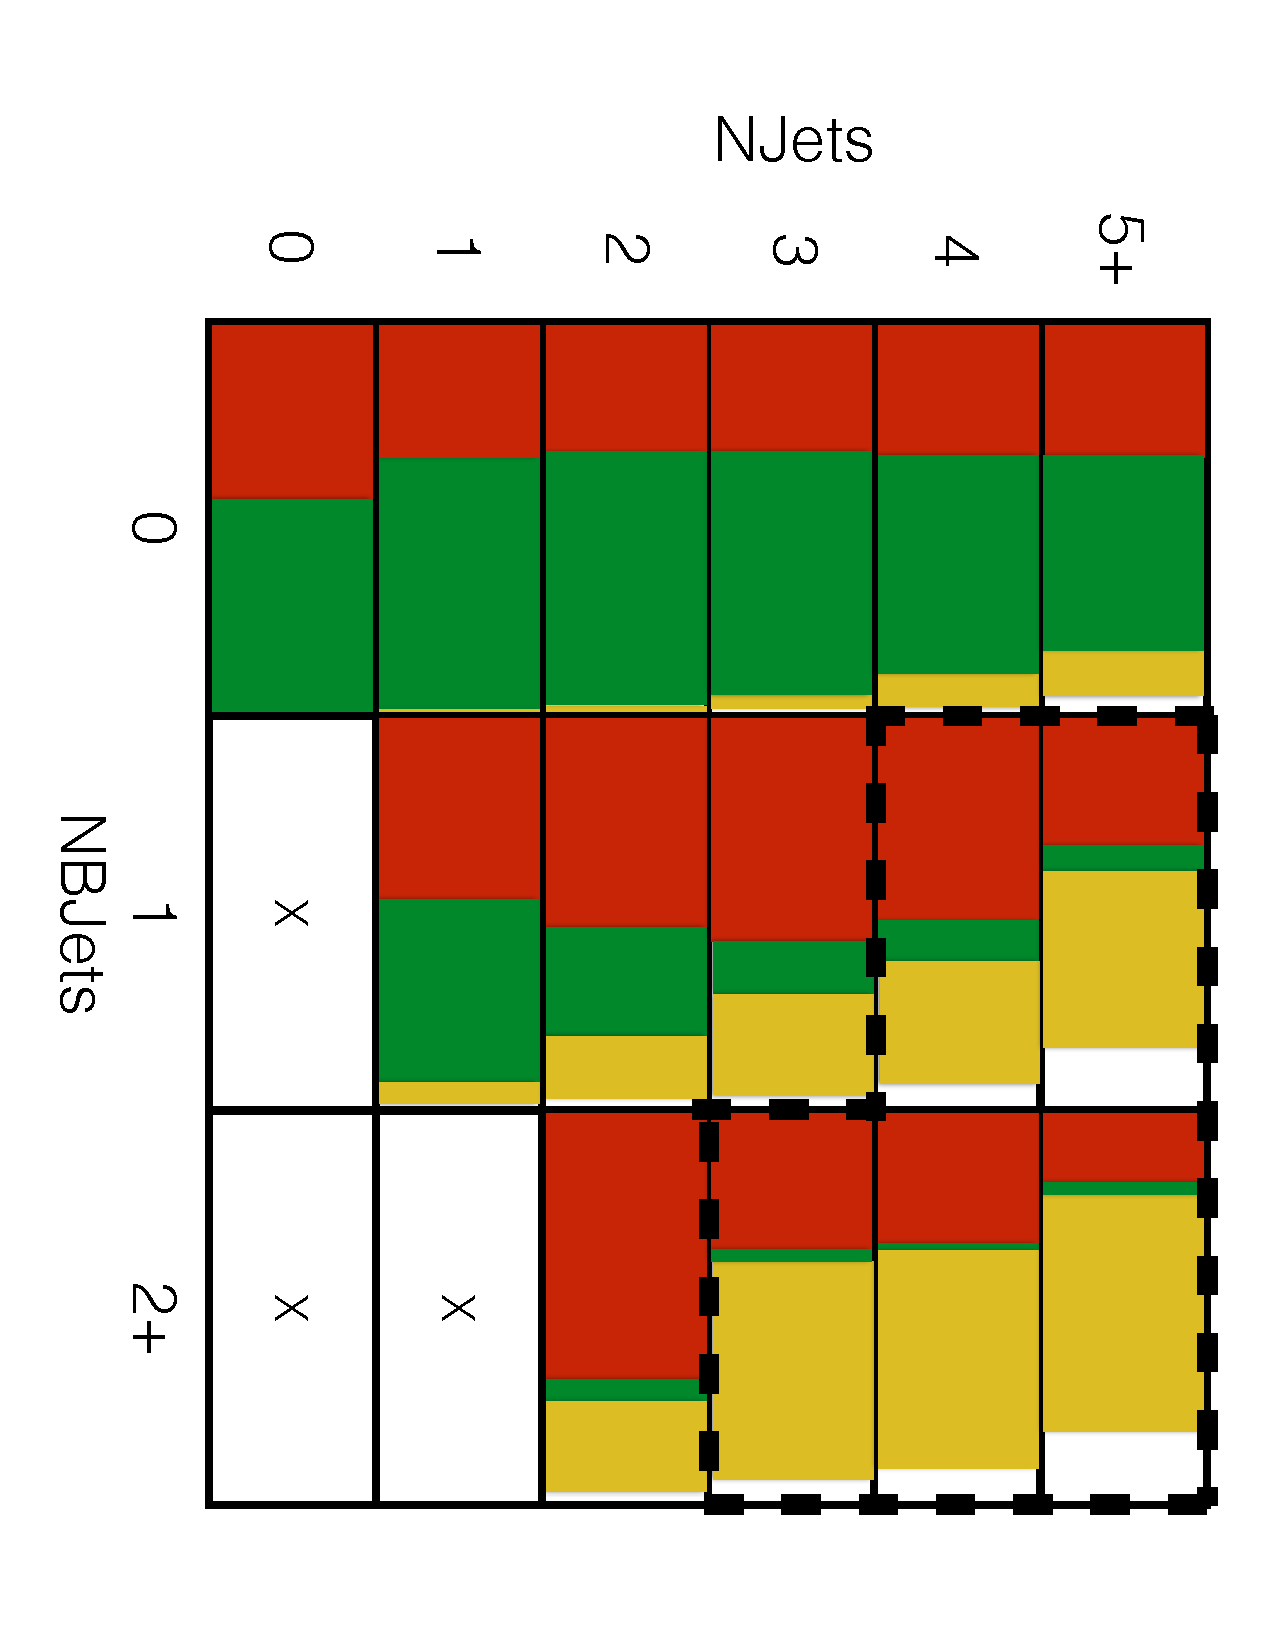
\includegraphics[angle=90,width=0.32\textwidth]{figs/selection/3l_selection.pdf}} &
\subfloat[4$\ell$]{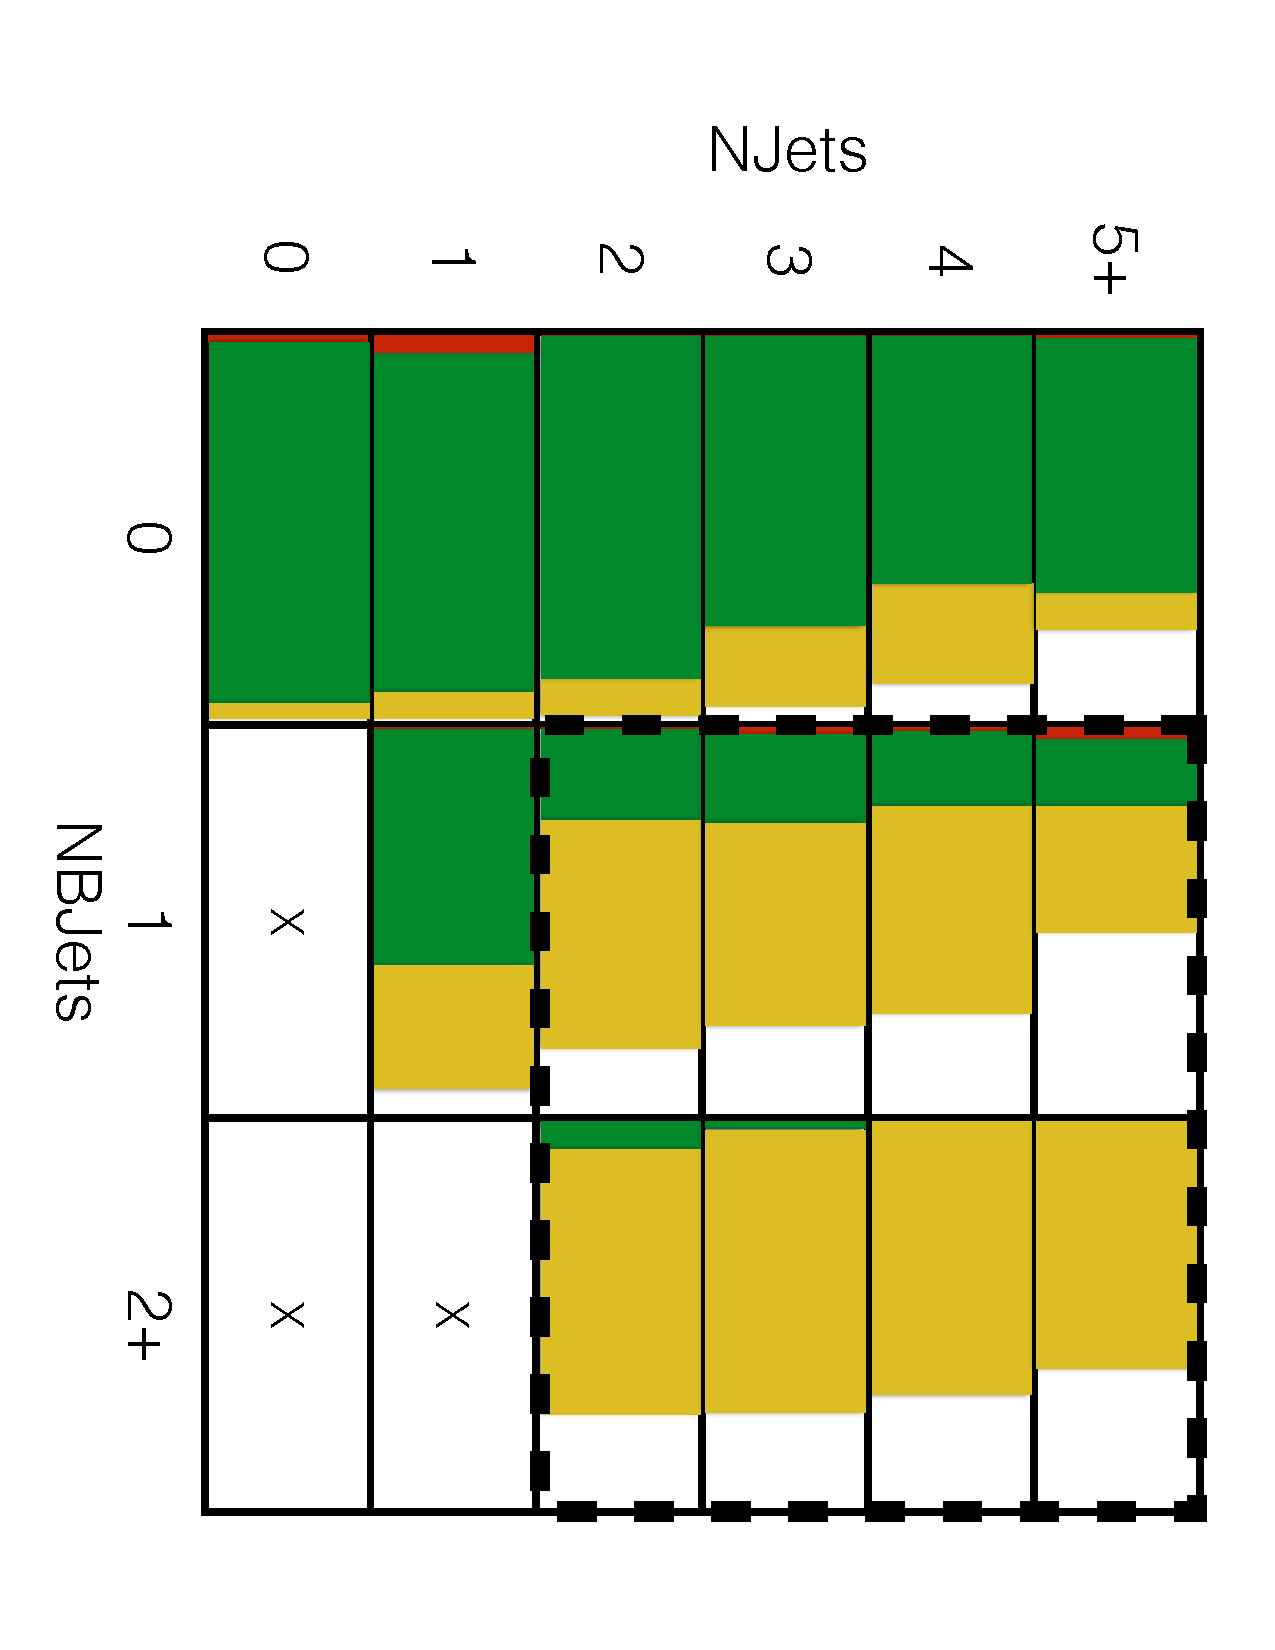
\includegraphics[angle=90,width=0.32\textwidth]{figs/selection/4l_selection.pdf}} \\
\multicolumn{3}{c}{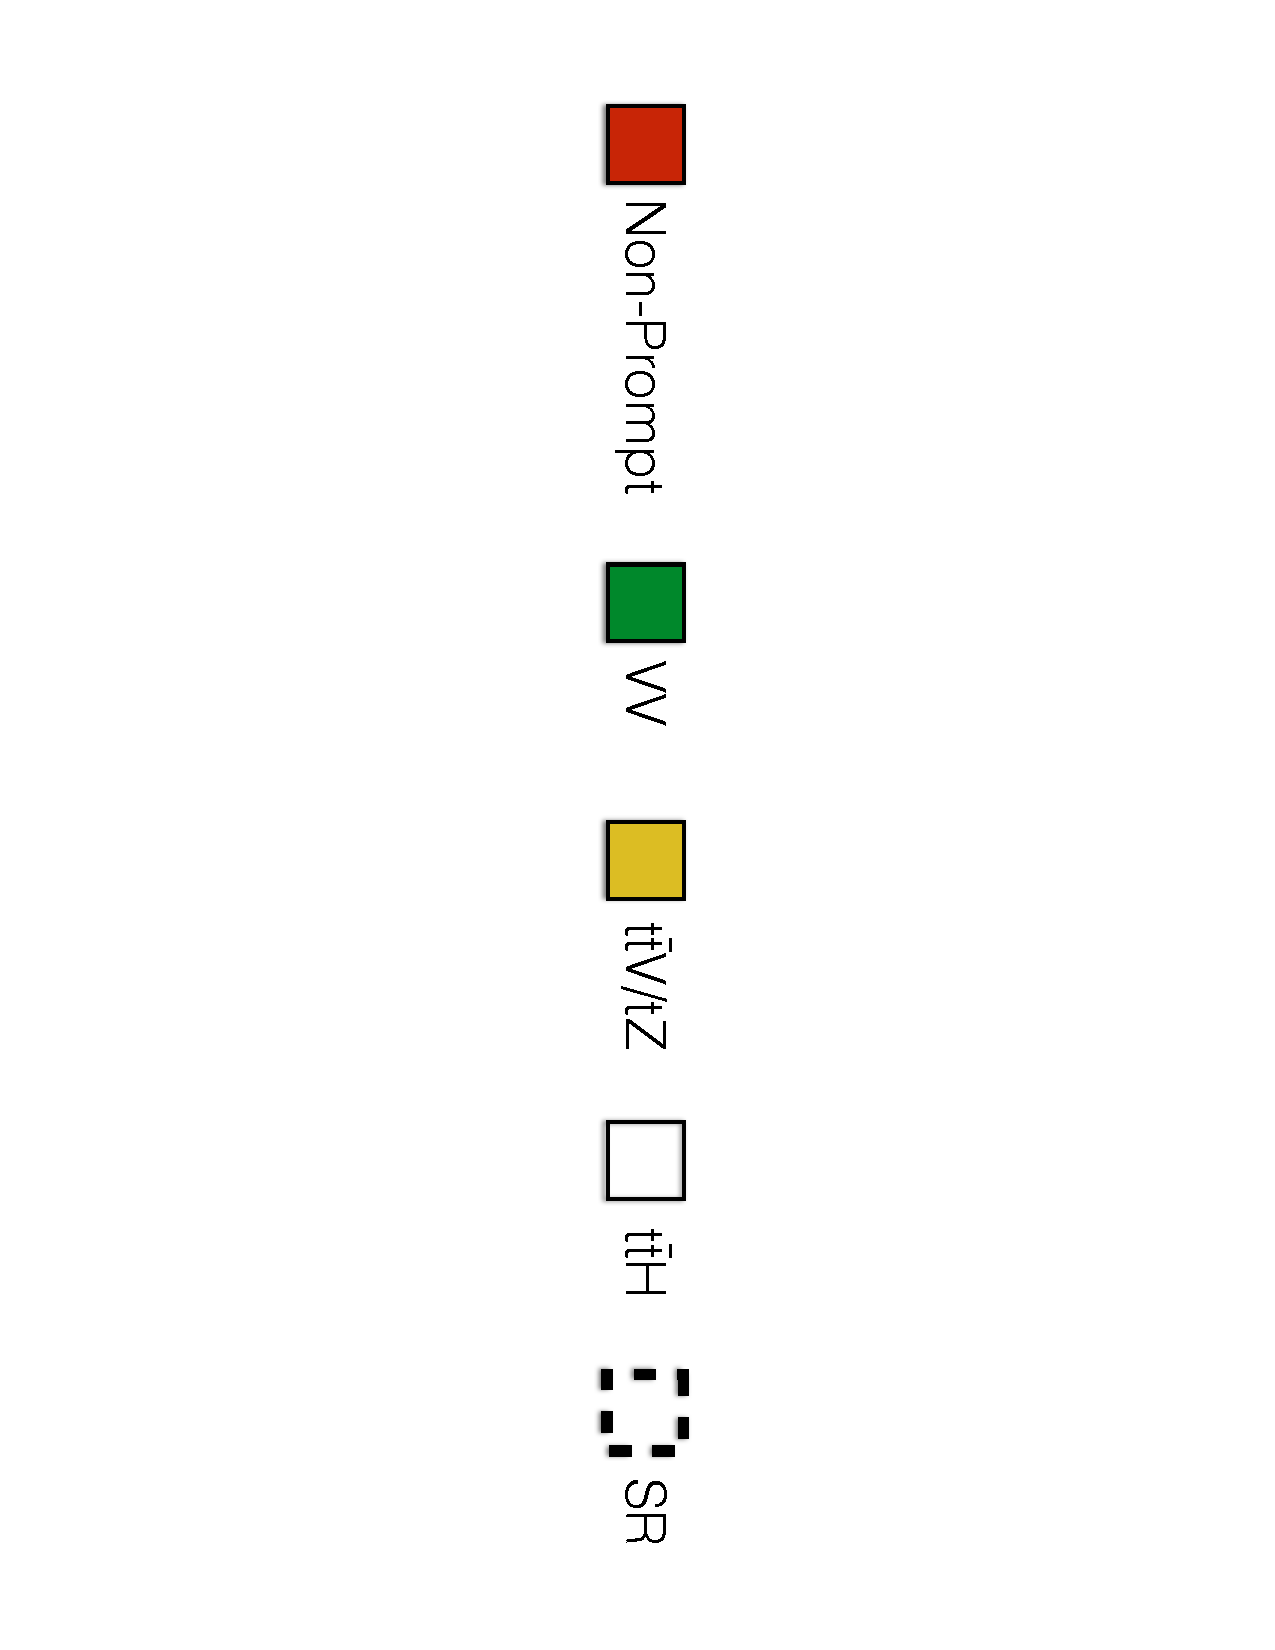
\includegraphics[angle=90,width=0.69\textwidth]{figs/selection/legend}} \\
\end{tabular} 
\caption{Number of jets vs. number of b-tagged jet plot for the fully selected multi-lepton channels. Signal regions
are outlined with a dashed line. Sub-channels are defined later in the 2$\ell$ SS and 4$\ell$ SRs. The fractional
background contribution to each jet and b-tagged jet bin are shown for non-prompt (red), \ttV $+$ \tZ\ (yellow), and $VV$ (green). The expected signal 
fraction is shown in white. The expected non-prompt fraction contains charge misidentifications and fakes. It is shown for MC only, although
data-based methods are used for the final result.
}
\label{figure:selection}
\end{figure}

\section{2$\ell$ Same-Charge Signal Region}

The 2 lepton signal region requires two leptons of similar charge (2$\ell$ SS). The signal is symmetric in charge but
the background from opposite-sign \ttbar\ di-lepton production would be overwhelming. Requiring
only two leptons allows the extra 2 W bosons in the event to decay hadronically, resulting in on average 4 additional
light jets plus 2 additional b-quark jets from the top decays. 

We require a leading lepton with transverse momentum of at least 25 GeV that matches to a
trigger and a sub-leading lepton of at least 20 GeV, a b-tagged jet, and at least 4 jets in
total.  

In order to suppress non-prompt backgrounds, the lepton isolation criteria for tracking and 
calorimeter are tightened from less than 10\% of the lepton momentum to 5\%. To suppress
charge misidentification, the electron is required to be extremely central ($|\eta| < 1.37$) 
to avoid the material-rich regions of the detector. Additionally, $ee$ events with a 
lepton pair invariant mass within 10 GeV of the Z pole are removed. To maintain orthogonality with the $\tau$ analyses, events with fully identified
taus are vetoed.

For the statistical combination the channel is divided into 6 sub-channels:
2 jets counting bins (N$_{Jet}$ $=$ 4, N$_{Jet}$ $\geq$ 5) x 3 lepton flavor bins (ee,$\mu\mu$,e$\mu$). 


\section{3$\ell$ Signal Region}

The 3 lepton channel requires 3 leptons, whose summed charge is either
$-$1 or $+$1. The leptons are ordered in this way:

\begin{itemize}
\item \textbf{lep0:} the lepton that is opposite in charge to the other two leptons
\item \textbf{lep1:} the lepton that is closer in $\Delta R$ to lep0
\item \textbf{lep2:} the lepton that is farther in $\Delta R$ from lep1
\end{itemize}

Since events with a fake lepton arise exclusively from opposite sign di-lepton processes, \ttbar\ and Z+jets, where additional jets are 
misidentified as the third lepton, lep0 is never the fake lepton. As a result, the transverse momentum 
requirement of lep0 ($> 10$ GeV) is lower that the other two, $>$ 20 GeV.  One lepton must
must match a trigger and have $p_T >$ 25 GeV. 

The 3$\ell$ channel further requires at least one b-tagged jet and at least 4 jets in total, or two b-tagged jets and exactly 3 jets in 
total. Additionally, to suppress \WZ\ and \zj events, events with same-flavor opposite-sign (SFOS) pairs
within 10 GeV of the $Z$ pole are vetoed.

Additional cuts, including a di-lepton mass cut, and splittings were investigated but low statistics proved to wash out any advantages.
The di-lepton mass cut will be a useful discriminator in future analyses since the spin statistics of Higgs decay in $W$ bosons often
causes the two emitted opposite-sign leptons to point in the same direction, resulting in a small measured invariant mass. 

\section{4$\ell$ Signal Region}

In the four lepton signal region, selected events must have exactly four leptons with a total charge of zero. 
At least one lepton must be matched to one of the applied single lepton trigger and have a transverse momentum above 25 GeV. 
The leading and sub-leading leptons are required to have transverse momentum of 25 and 15 GeV respectively. 
In order to suppress background contributions from low-mass resonances and Drell-Yan radiation, all SFOS lepton pairs are required to have a dilepton invariant mass of at least 10 GeV. 

The four-lepton invariant mass is required to be between 100 and 500 GeV. 
This choice of mass window suppresses background from the on-shell $Z\to4\ell$ peak and exploits the high-mass differences between the signal and the dominant \ttZ\ background. 
Events containing an SFOS lepton pair within 10 GeV of the Z boson mass are discarded. 
This Z-veto procedure greatly reduces background contributions from \ZZ and \ttZ. 
Finally, selected events are required to have at least two jets, at least one of which must be tagged as a b-quark jet.  

The contribution from \ttZ\ comprises approximately 75\% of the total background in the inclusive signal region. 
A signal region categorization which factorizes \ttZ\ from the remaining backgrounds is thus beneficial. 
The signal region is accordingly divided into two categories based on the presence of SFOS lepton pairs in the final state. 

\section{Electron Selection}

The electrons are reconstructed by a standard algorithm of the
experiment~\cite{ATLAS-CONF-2014-032} and the electron cluster is required to be fiducial 
to the barrel or endcap calorimeters: $|\eta_{cluster}| < $ 2.47. Electrons
in the transition region, $1.37 < |\eta_{cluster}| < 1.52$, are vetoed.
Electrons must have \pt$>$10 GeV and pass the \textsc{verytight} likelihood identification criteria.

In order to reject jets misidentified as electrons,
electron candidates  must also be well isolated from additional tracks and
calorimeter energy around the electron cluster. Both the tracking 
and calorimeter energy within $\Delta R=0.2$ of the electron
cluster must be less than 5\% of the electron transverse momentum: ptcone20/P$_T <$ 0.05 and Etcone20/E$_T <$ 0.05.
All quality tracks with momentum greater than 400 MeV contribute to the isolation
energy.  Calorimeter isolation energy is calculated
using topological clusters with corrections for energy leaked from the
electron cluster. Pile-up and underlying event corrections are applied using
a median ambient energy density correction.  

The electron track must also match the primary vertex. The longitudinal projection 
of the track along the beam line, $z0\sin{\theta}$, must be less than 1 cm) and the transverse projection divided by the
parameter error, $d0$ significance, must be less than 4. These cuts are used in particular to suppress backgrounds
from conversions, heavy-flavor jets and electron charge-misidentifications. 


The electron selection is summarized in Table~\ref{selection:table_object}. 


\section{Muon Selection}

Muons used in the analysis are formed by matching reconstructed inner detector
tracks with either a complete track or a track-segment reconstructed in the muon spectrometer (MS),
called Chain 2 muons. The muons have \pt$>$10 GeV and satisfy $|\eta| < 2.5$.
The muon track are required to be a good quality combined fit of inner detector hits and muon
spectrometer segments, unless the muon is not fiducial to the
inner detector, $|\eta| > 2.47$.  Muons with inner detector tracks are further required
to pass standard inner detector track hit requirements~\cite{MCP2012}.  

As with electrons, muons are required to be isolated from 
additional tracking or calorimeter energy: ptcone20/P$_T <$ 0.1, Etcone20/E$_T <$ 0.1. A cell-based Etcone20/P$_T$ relative
isolation variable is used. A pile-up energy subtraction based 
on the number of reconstructed vertices in the event is applied. The
subtraction is derived from a Z boson control sample.


The muons must also originate from the primary vertex and have impact parameter requirements, $d0$ significance $<$ 3, and $z0\sin{\theta} <$ 0.1 cm, similar to the electrons. 


The muon selection is summarized in Table~\ref{selection:table_object}. 

\section{Jet and b-Tagged Jet Selection}

Jets are reconstructed in the calorimeter using the anti-$k_t$~\cite{Cacciari:2008gp} algorithm
with a distance parameter of 0.4 using locally calibrated
topologically clusters as input (LC Jets). Since the jets in the \tth\
signal mostly arise from the decay massive resonances and not radiation,
they are expected to be central and high energy. Jets must have \pt$>$25 GeV and 
$|\eta|<2.5$. 

Jets must also pass loose quality requirement, ensuring the proper
functioning of the calorimeter at the time of data taking. Jets near a hot calorimeter cell in data periods
B1/B2 are rejected. The local hadronic calibration is used for
the jet energy scale, and ambient energy corrections are applied to account
for energy due to pileup.

Jets within $|\eta| < 2.4$ and $p_T <$ 50 GeV are further required to be
associated with the primary vertex. The the fraction of track $p_T$ associated with the jet that comes from the primary vertex,
must exceed 0.5 (or there must be no track associated to the jet). This requirement rejects jets that arise from pile-up 
vertices.

B-jets are tagged using a Multi-Variate Analysis (MVA) method called MV1 and relying on information
of the impact parameter and the reconstruction of the displaced vertex of the
hadron decay inside the jet\cite{ATLAS-CONF-2011-102}.
The output of the tagger is required to be above 0.8119 which corresponds to a $70\%$ efficient Working Point (WP).

\section{Object Summary and Overlap}

Since many fully identified objects may be reconstructed as two different objects, an overlap removal procedure is applied.
Electrons within $\Delta R < 0.1$ of muons are rejected in favor of the muon. Jets within $\Delta R < 0.3$ of electrons are 
then removed. Finally, muons within $\Delta R < 0.04 + 10 GeV/p_{T}$ of jets are rejected, as these muons are thought to
arise from jet fragmentation. 

\begin{table}[htbp]
  \begin{center}
    {\small
    \begin{tabular}{l|c|c}
      \hline
      Parameter     &  Values & Remarks \\
      \hline
      \multicolumn{3}{c}\textbf{Electrons}\\
      \hline
      \pt~ & $>10~\GeV$ & \\ 
      $|\eta|$~ & $< 2.47 $ veto crack & $<1.37$ for 2$\ell$ SS channel \\ 
      ID & Very Tight Likelihood &  \\ \hline
      Isolation & \etrel,\ptrel $<0.05$   &   \\ \hline
      Jet overlap removal & $\Delta R>0.3$  &  \\ \hline
      $|d_0^{\rm sig}|$ & $<4\sigma$  &  \\ \hline
      $z_0 sin\theta$ & $<1~cm$   &   \\ \hline\hline

      \multicolumn{3}{c}\textbf{Muons}\\
      \hline
      \pt~ & $>10~\GeV$ & \\ 
      $|\eta|$~ & $< 2.5 $ \\ 
      ID & Tight &  \\ \hline
      Jet overlap removal & $\Delta R>0.04+10\GeV/p_{T}$  &  \\ \hline
      Isolation & \etrel,\ptrel $<0.1$  & $<0.05$ for 2 leptons \\ \hline
      $|d_0^{\rm sig}|$ & $<3\sigma$  &  \\ \hline
      $z_0$ & $<1~cm$   &   \\ \hline\hline
      \multicolumn{3}{c}\textbf{Jets}\\
      \hline
      \pt~ & $>25\GeV$ &  \\ \hline
      $|\eta|$ & $<2.5$ &  \\ \hline
      JVF & JVF$>0.5$ or no associated track or \pt$>50~{\rm GeV}$ &  \\ \hline\hline
      b-Tag & MV1 70\% operating point&  \\ \hline\hline
    \end{tabular}
    }
    \caption{\label{tab:obj-final} Object identification and selection used to define the 5 channels of the
    multi-lepton \tth\ analysis. Some channels use a sub-sample of objects as
    explained in the Remarks column.}
    \label{selection:table_object} 
  \end{center}
\end{table}


